\documentclass[11pt,a4paper]{article}

\usepackage[margin=1in]{geometry}
\usepackage[T1]{fontenc}
\usepackage[utf8]{inputenc}
\usepackage{lmodern}
\usepackage{graphicx}
\usepackage{booktabs}
\usepackage{longtable}
\usepackage{array}
\usepackage{caption}
\usepackage{hyperref}
\usepackage{pgfplots}
\usepackage{float}
\usepackage{enumitem}

\pgfplotsset{compat=1.18}
\hypersetup{colorlinks=true,linkcolor=blue,urlcolor=blue,citecolor=blue}
\setlength{\emergencystretch}{2em}
\setlist[itemize]{noitemsep,topsep=3pt}

\title{IIT Jodhpur Academic Helpdesk\\[0.35em]
\large Multi-Agent System and Evaluation}
\author{Shashank Parchure (B23CM1059)\\
Soham Laxman Khairnar (B23CM1039)\\
Saher Dev (B23CS1059)\\
Sarthak Kolekar (B23CS1065)}
\date{Evaluation reviewed 29 October 2026}

\begin{document}
\maketitle

\begin{abstract}
We built a local academic helpdesk for IIT Jodhpur that uses Google ADK, Ollama, ChromaDB, and institute documents. A multi-agent version routes requests to policy, schedule, and email specialists. The main evaluation used 28 prompts: 20 about academic matters and 8 outside the helpdesk's scope. Qwen3 8B was run twice on the same prompt set. The team marked 16 of 20 academic answers correct in the first run and 12 of 20 in the second; citations were marked correct for 18 of 20 in each run. All 16 out-of-scope questions were logged. The entered refusal grades were 4 of 8 in Run 1 and 8 of 8 in Run 2, although the Run 1 answers marked incorrect also contain explicit refusals. A separate 14-prompt experiment compared Qwen3 8B and Llama 3.1 8B. Qwen3 had higher answer accuracy on the graded subset (12/20 versus 8/19), while citation results were close. Repeated runs produced several substantial changes, most often between answering from evidence and abstaining. The team reports no unsupported claims across the reviewed outputs. The results show that the system can answer exact timetable and course questions, but document retrieval and answer stability still need improvement.
\end{abstract}

\tableofcontents
\newpage

\section{Project goal}

The assignment asks for an IIT Jodhpur academic helpdesk that can answer questions about programmes, courses, rules, timetables, and instructor contacts; draft an email without sending it; cite the source used; and log questions it cannot answer. Requests outside that scope should receive a refusal rather than a guessed answer.

The project retains the original single-agent app as a baseline and adds a separate multi-agent app. This report focuses on the multi-agent system, as required for the main evaluation. The screenshots in Section~\ref{sec:screenshots} show the ADK interface while the single-agent app answered a related credit question.

The code repository, evaluation prompts, and supporting project files are available at \url{https://github.com/shashankparchure/Academic-Helpdesk-Agent}.

\section{System overview}

\subsection{Data and retrieval}

The source material is collected under \texttt{data/raw}. The preparation scripts extract text from documents, export workbook sheets, use manually extracted text for scanned PDFs, and normalize course offerings, classroom allocations, and slot times into CSV tables. The source register stores document identifiers and paths used for citations.

The existing local retrieval stack uses Ollama's \texttt{qwen3-embedding:0.6b} embedding model and a persistent ChromaDB collection. Questions are embedded locally; nearby chunks are retrieved with their citation metadata and passed to the agent. Structured tools provide exact course and timetable lookups, course counts, faculty email lookup, email drafting, and logging of unanswered questions. The email tool prepares a draft only; it does not send mail. The evaluation used the existing vector index and did not rebuild it between runs.

\subsection{Agents}

The multi-agent app has an orchestrator and three specialists:
\begin{itemize}
  \item \textbf{Policy specialist:} curriculum, academic regulations, registration, examination, and credit questions.
  \item \textbf{Schedule specialist:} course codes, course offerings, slots, classroom allocations, and timetable details.
  \item \textbf{Email specialist:} course instructor lookup, faculty contact lookup, and draft preparation.
\end{itemize}
The orchestrator handles clearly out-of-scope questions and records them for follow-up. The baseline and multi-agent apps use the same underlying data and retrieval tools so that changing the chat model does not also change the knowledge base.

\section{Evaluation design}

\subsection{Main Qwen3 evaluation}

The main evaluation used the complete 28-prompt set in \texttt{eval/evaluation\_prompts.txt} and \texttt{eval/prompts.json}. It contains four groups of seven prompts, one group per contributor. Five prompts in each group are academic and two are outside the helpdesk scope, giving 20 in-scope and 8 out-of-scope questions. Qwen3 8B was run twice with the same set and existing index. The two runs are stored under \texttt{eval/results/all\_prompts/multi\_qwen3\_8b\_28q/}.

\subsection{Model replacement subset}

For the model comparison, the team used the earlier matched 14-prompt subset: seven prompts from Soham's set and seven from Sarthak's set. Qwen3 8B and Llama 3.1 8B each ran this subset twice through the multi-agent app. These are separate from the main 28-prompt evaluation, and their results are retained under \texttt{eval/results/multi\_qwen3\_8b/} and \texttt{eval/results/multi\_llama3\_1\_8b/}.

\subsection{Scoring}

The summary sheets contain manual grades. Answer accuracy is measured only on in-scope prompts; an answer counts when it addresses the request with the expected facts. Citation correctness is scored separately, since an answer can be right but poorly sourced, or cite a relevant document without answering. For out-of-scope prompts, refusal and follow-up logging are separate measures. A response that declines the request but fails to log it can receive a correct refusal and an incorrect logging result.

The team reviewed the outputs and reports no unsupported claims across the 112 response records (0/112). The \texttt{unsupported\_claims} cells are blank in the CSV files, so this is a team-level review result rather than a computed CSV percentage. The analysis of answer changes compares the substance of each final answer across runs; small wording changes are not counted.

\section{Main evaluation: Qwen3 on 28 prompts}

\subsection{Scores}

Table~\ref{tab:main-qwen} summarizes the entered grades. Each run contains 20 in-scope and 8 out-of-scope answers.

\begin{table}[htbp]
\centering
\caption{Qwen3 results on the full 28-prompt set.}
\label{tab:main-qwen}
\begin{tabular}{lrrrr}
\toprule
Run & \shortstack{Answer\\accuracy} & \shortstack{Citation\\correctness} & \shortstack{Correct\\refusal} & \shortstack{Follow-up\\logging} \\
\midrule
Run 1 & 16/20 (80\%) & 18/20 (90\%) & 4/8 (50\%) & 8/8 (100\%) \\
Run 2 & 12/20 (60\%) & 18/20 (90\%) & 8/8 (100\%) & 8/8 (100\%) \\
Pooled & 28/40 (70\%) & 36/40 (90\%) & 12/16 (75\%) & 16/16 (100\%) \\
\bottomrule
\end{tabular}
\end{table}

The answer score fell by four questions between runs. Citation correctness stayed at 18 of 20 in both runs. Every out-of-scope question was logged in both runs. The submitted refusal grades improved from 4/8 to 8/8. Figure~\ref{fig:group-accuracy} shows the participant-group breakdown; the largest drop is in Saher's in-scope score, while Shashank's score is unchanged.

The in-scope scores by participant group show where the second run changed most:
\begin{center}
\small
\begin{tabular}{lrrrr}
\toprule
Group & Answer Run 1 & Answer Run 2 & Citation Run 1 & Citation Run 2 \\
\midrule
Soham & 4/5 & 3/5 & 4/5 & 5/5 \\
Shashank & 4/5 & 4/5 & 4/5 & 4/5 \\
Saher & 4/5 & 2/5 & 5/5 & 4/5 \\
Sarthak & 4/5 & 3/5 & 5/5 & 5/5 \\
\bottomrule
\end{tabular}
\end{center}

There is a scoring detail to check before the final submission. In Run 1, the four out-of-scope responses in Saher's and Sarthak's sets are marked incorrect refusals, but their text explicitly declines the request and does not provide the requested restaurant, travel, recipe, or sports prediction. The Run 1 responses in Soham's and Shashank's sets are marked correct. The results above preserve the CSV grades; if all explicit declines meet the team's refusal rubric, the pooled refusal result would instead be 16/16. The team should settle this rubric point and update the sheet consistently.

% Summary charts for report.tex. Run scripts/generate_report_figures.py to refresh.
\begin{figure}[htbp]
\centering
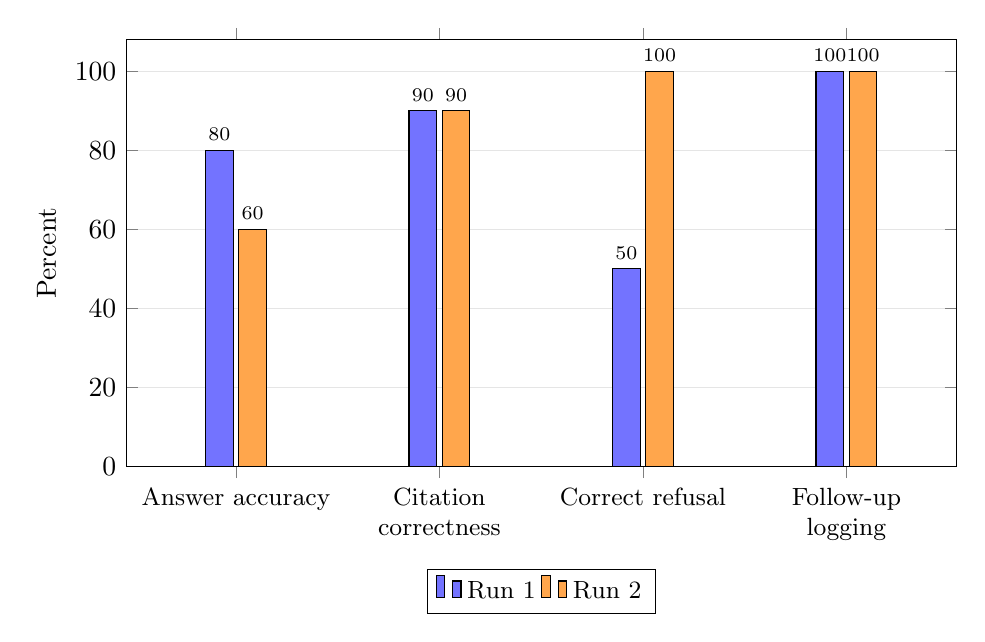
\begin{tikzpicture}
\begin{axis}[
  ybar, bar width=10pt, width=\textwidth, height=7cm,
  ymin=0, ymax=108, ylabel={Percent},
  symbolic x coords={accuracy,citation,refusal,logging}, xtick=data,
  xticklabels={Answer accuracy,Citation correctness,Correct refusal,Follow-up logging},
  x tick label style={text width=2.4cm,align=center,font=\small},
  ymajorgrids=true, grid style={gray!20},
  nodes near coords, nodes near coords style={font=\scriptsize},
  enlarge x limits=0.18,
  legend style={at={(0.5,-0.24)},anchor=north,legend columns=2,font=\small},
]
\addplot[fill=blue!55] coordinates {(accuracy,80) (citation,90) (refusal,50) (logging,100)};
\addlegendentry{Run 1}
\addplot[fill=orange!70] coordinates {(accuracy,60) (citation,90) (refusal,100) (logging,100)};
\addlegendentry{Run 2}
\end{axis}
\end{tikzpicture}
\caption{Qwen3 on the main 28-prompt set. Accuracy and citation correctness use 20 in-scope prompts per run; refusal and logging use eight out-of-scope prompts. Refusal bars use the entered CSV grades.}
\label{fig:qwen-main}
\end{figure}

\begin{figure}[htbp]
\centering
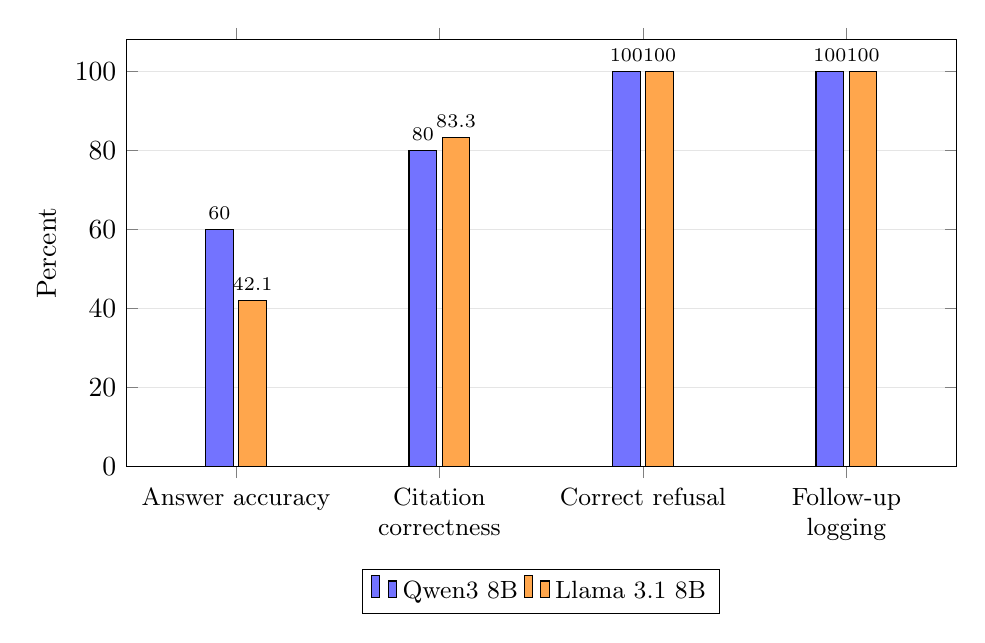
\begin{tikzpicture}
\begin{axis}[
  ybar, bar width=10pt, width=\textwidth, height=7cm,
  ymin=0, ymax=108, ylabel={Percent},
  symbolic x coords={accuracy,citation,refusal,logging}, xtick=data,
  xticklabels={Answer accuracy,Citation correctness,Correct refusal,Follow-up logging},
  x tick label style={text width=2.4cm,align=center,font=\small},
  ymajorgrids=true, grid style={gray!20},
  nodes near coords, nodes near coords style={font=\scriptsize},
  enlarge x limits=0.18,
  legend style={at={(0.5,-0.24)},anchor=north,legend columns=2,font=\small},
]
\addplot[fill=blue!55] coordinates {(accuracy,60) (citation,80) (refusal,100) (logging,100)};
\addlegendentry{Qwen3 8B}
\addplot[fill=orange!70] coordinates {(accuracy,42.1) (citation,83.3) (refusal,100) (logging,100)};
\addlegendentry{Llama 3.1 8B}
\end{axis}
\end{tikzpicture}
\caption{Pooled results on the matched 14-prompt LLM subset, two runs per model. Percentages use nonblank grades; the Llama answer and citation rates therefore have smaller denominators.}
\label{fig:llm-subset}
\end{figure}

\begin{figure}[htbp]
\centering
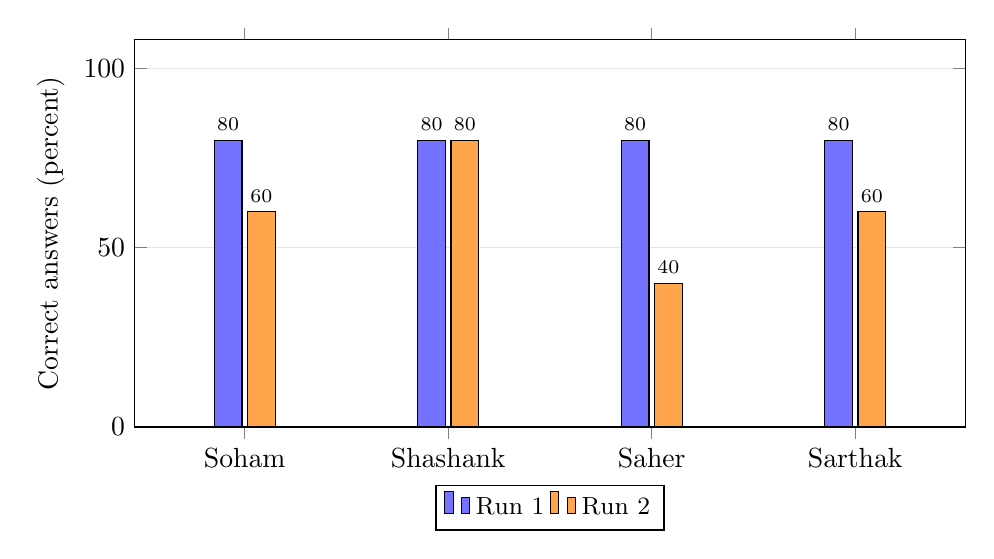
\begin{tikzpicture}
\begin{axis}[
  ybar, bar width=10pt, width=\textwidth, height=6.5cm,
  ymin=0, ymax=108, ylabel={Correct answers (percent)},
  symbolic x coords={soham,shashank,saher,sarthak}, xtick=data,
  xticklabels={Soham,Shashank,Saher,Sarthak},
  ymajorgrids=true, grid style={gray!20},
  nodes near coords, nodes near coords style={font=\scriptsize},
  enlarge x limits=0.18,
  legend style={at={(0.5,-0.15)},anchor=north,legend columns=2,font=\small},
]
\addplot[fill=blue!55] coordinates {(soham,80) (shashank,80) (saher,80) (sarthak,80)};
\addlegendentry{Run 1}
\addplot[fill=orange!70] coordinates {(soham,60) (shashank,80) (saher,40) (sarthak,60)};
\addlegendentry{Run 2}
\end{axis}
\end{tikzpicture}
\caption{Correct-answer rate by participant group on the main Qwen3 prompt set. Each group has five in-scope questions.}
\label{fig:group-accuracy}
\end{figure}


\subsection{What worked and where answers varied}

Timetable answers were the most stable examples. The model returned the Autonomous Systems slot and EEL7080 schedule in both main runs, with citation grades marked correct. It also consistently answered the 400-level Humanities question by explaining that the available course data did not identify a Humanities department sheet clearly enough to count. The reviewer marked that response correct in Run 1 but not in Run 2, and marked its citation incorrect in Run 2, so this item merits a quick grading check.

The main instability was retrieval-dependent. On some questions, one run retrieved enough content to answer and the other returned only a document title or said that the excerpt did not expose the relevant content. The clearest cases were the course overload guidelines, Minor Examination rules, the SoLA course count, and the BS Chemistry curriculum. Email drafting also varied: one run drafted the requested EEL4330 email, while the other asked for the student's name before drafting.

\section{LLM replacement experiment: 14-prompt subset}

\subsection{Scores}

The model comparison used the same 14 questions for both models. Table~\ref{tab:model-subset} pools the two runs. Blank grades are excluded from the answer and citation denominators.

\begin{table}[htbp]
\centering
\caption{Qwen3 and Llama 3.1 on the matched 14-prompt subset.}
\label{tab:model-subset}
\begin{tabular}{lrrrr}
\toprule
Model & \shortstack{Answer\\accuracy} & \shortstack{Citation\\correctness} & \shortstack{Correct\\refusal} & \shortstack{Follow-up\\logging} \\
\midrule
Qwen3 8B & 12/20 (60\%) & 16/20 (80\%) & 8/8 (100\%) & 8/8 (100\%) \\
Llama 3.1 8B & 8/19 (42.1\%) & 15/18 (83.3\%) & 8/8 (100\%) & 8/8 (100\%) \\
\bottomrule
\end{tabular}
\end{table}

Llama has one ungraded answer and two ungraded citation rows. If its blank answer grade were treated as incorrect, its accuracy would be 8/20 (40\%). The entered scores favor Qwen3 on answer correctness by about 18 percentage points. Citation scores are close; Llama's higher scored percentage is based on fewer graded rows. Both models received full marks for refusal and logging on this subset. With only 14 questions and two repeats, these results are useful for choosing what to investigate, not for claiming a general model ranking.

The Llama run 2 CSV contains the literal value \texttt{no} in one \texttt{error} cell for the overload question, while the answer is present and there is no error message. This is treated as a manual ``no error'' entry, not a failed run; the cell should be cleared or moved to its intended grading column before archiving the data.

\section{Substantial answer changes across runs}

Only changes in the substance of the answer are listed here. Rephrasing, formatting, or adding a citation without changing the answer is not counted. The main Qwen results use the 28-prompt set. The two subset comparisons refer to the older matched 14-prompt set.

\subsection{Main Qwen3 run: 28 prompts}

\begin{itemize}
  \item \textit{What do the current course overload guidelines say about taking credits beyond the normal load?} Responses ranged from a summary of overload rules to an abstention because the retrieved excerpt contained only document metadata.
  \item \textit{What rules apply to the Minor Examination in Semester I of Academic Year 2026-27?} One response said the rules were unavailable; another summarized the examination guidance.
  \item \textit{How many level-4 courses are listed under the School of Liberal Arts (SoLA), and which are explicitly identified as electives?} One response counted six courses and said none were explicitly identified as electives; another could not access the required data.
  \item \textit{Draft an email to the instructor of EEL4330 requesting two days of sick leave. Include the contact source and citation, and do not send the email.} One response provided a draft; another asked for the student's name without drafting it.
  \item \textit{According to the BS Chemistry curriculum document, what programme requirements should a student complete to graduate?} Responses ranged from a programme-requirements summary to an abstention because the retrieved excerpt did not contain the curriculum details.
\end{itemize}

The Open Elective answer is not listed as a substantial change because both responses state 10 credits. Both responses to the Major Examination attendance question also abstained, and the out-of-scope answers continued to refuse despite wording differences.

\subsection{Qwen3 on the 14-prompt subset}

\begin{itemize}
  \item \textit{How many Open Elective credits are required to earn a B.Tech. degree?} One response could not find a value; another answered 10 credits.
  \item \textit{Draft an email to the instructor of CSL7650 requesting sick leave for two days. Use the instructor and contact details from the supplied data, cite the sources, and do not send the email.} One response asked for more student details; another provided a complete draft.
  \item \textit{According to the BS Chemistry curriculum document, what programme requirements should a student complete to graduate?} A document-title-only response changed to a curriculum summary.
  \item \textit{What change is described in the 28 Credit Revision dated 11 January 2024?} One response could not retrieve the revision; another said the requirement fell from 20 to 15 credits.
  \item \textit{Has B.Tech. branch change been discontinued for Academic Year 2026-27? Reconcile the current discontinuation circular with any older branch-change guidance and cite both if relevant.} One response gave the policy conclusion; another abstained because relevant evidence was not retrieved.
\end{itemize}

\subsection{Llama 3.1 on the 14-prompt subset}

\begin{itemize}
  \item \textit{What attendance requirement must a student meet to sit in the Major examination?} One response gave Minor Examination attendance rules; another returned unrelated citation and grade metadata. Neither answered the Major Examination question.
  \item \textit{How many Open Elective credits are required to earn a B.Tech. degree?} Responses shifted from a generic curriculum-document overview to a discussion of B.Tech. specializations. Neither gave the requested Open Elective credit value.
  \item \textit{What slot is assigned to the course Autonomous Systems? Cite the course-list source.} A response based on an incorrect schedule-tool result differed from a direct slot E answer using the course-list source.
  \item \textit{What do the current course overload guidelines say about taking credits beyond the normal load?} A summary of overload rules differed from an unrelated explanation of citation metadata.
  \item \textit{Draft an email to the instructor of CSL7650 requesting sick leave for two days. Use the instructor and contact details from the supplied data, cite the sources, and do not send the email.} One response said an email had been drafted but did not show it; another included the draft.
  \item \textit{According to the BS Chemistry curriculum document, what programme requirements should a student complete to graduate?} Responses shifted from a curriculum summary to an explanation of citation metadata.
  \item \textit{What change is described in the 28 Credit Revision dated 11 January 2024?} A citation-metadata response differed from a summary of the reduction from 20 to 15 credits.
  \item \textit{Has B.Tech. branch change been discontinued for Academic Year 2026-27? Reconcile the current discontinuation circular with any older branch-change guidance and cite both if relevant.} A speculative summary of older rules differed from a direct answer that branch change was discontinued for AY 2026--27.
\end{itemize}

These changes point to instability in retrieval and response handling. They do not all indicate the same kind of error: some are changes from a refusal to an answer, some are a change in factual conclusion, and others are a change from a tool or metadata dump to a usable response.

\section{Interpretation and limitations}

The multi-agent system performed well on exact schedule lookups and logging. Its main weakness was not lack of documents alone: the same prompt sometimes received a usable excerpt in one run and only a title or unrelated metadata in another. Specialist routing and final answer handling also matter. The email agent sometimes asked for a name that could have been left as a placeholder, and Llama occasionally surfaced citation metadata instead of answering.

The main Qwen result should be reported separately from the model-subset experiment. The main set has 28 prompts and is the assignment's primary evaluation. The 14-prompt experiment is a smaller, matched comparison of two LLMs. Pooling the two would mix different prompt sets and answer a different question.

Several limitations should accompany any conclusion:
\begin{itemize}
  \item The main evaluation covers 28 prompts and two runs. It is a useful course project evaluation, not a broad reliability estimate.
  \item Answer and citation grades were entered manually. Llama has three blank grades; the main refusal labels in Qwen Run 1 appear inconsistent with the text of four answers.
  \item Unsupported-claim results come from the team's review statement, not populated per-row CSV grades.
  \item The run folders do not record retrieval latency or a source-index revision. No latency comparison is reported.
  \item The model experiment compares Qwen3 and Llama only on the 14-prompt subset. It does not compare the single-agent and multi-agent architectures quantitatively.
\end{itemize}

\section{Conclusion and next work}

On the full prompt set, Qwen3 answered 28 of 40 in-scope question instances correctly across two runs, with 36 of 40 citations marked correct. All 16 out-of-scope questions were logged. The entered refusal labels total 12 of 16, but four Run 1 labels should be reconciled with the explicit refusals in their answer text.

On the matched LLM subset, Qwen3 had higher answer accuracy than Llama 3.1 in the entered grades, while citation scores were close and both models received full refusal and logging scores. The small subset and missing Llama grades limit the strength of that comparison.

The next engineering pass should address retrieval of the exact policy or curriculum section, keep citations tied to supporting excerpts, and make email drafts complete when optional personalization is absent. The team should correct the refusal rubric labels and the remaining blank Llama grades, then preserve the 28-prompt Qwen scores as the primary result. The full question set and evaluation artifacts are included with the repository.

\section{ADK interface screenshots}
\label{sec:screenshots}

The following screenshots were supplied with the project. They document a single-agent ADK session about total B.Tech. credits: the submitted question and retrieval activity, a citation result, and the final answer. They are included as implementation evidence and are not counted as multi-agent evaluation observations.

\begin{figure}[htbp]
\centering
\includegraphics[width=0.96\linewidth]{\detokenize{Screenshot 2026-10-17 082842.png}}
\caption{ADK web interface showing the B.Tech. credit question and source-search activity.}
\label{fig:adk-search}
\end{figure}

\begin{figure}[htbp]
\centering
\includegraphics[width=0.82\linewidth]{\detokenize{Screenshot 2026-10-17 082940.png}}
\caption{Retrieved academic-regulation excerpt and citation metadata shown in the ADK interface.}
\label{fig:adk-evidence}
\end{figure}

\begin{figure}[htbp]
\centering
\includegraphics[width=0.96\linewidth]{\detokenize{Screenshot 2026-10-17 083134.png}}
\caption{Final answer identifying 165 credits for the standard B.Tech. programme, with the cited regulation.}
\label{fig:adk-answer}
\end{figure}

\end{document}
